\documentclass[10pt,conference,compsocconf]{IEEEtran}

\usepackage{hyperref}
\usepackage{graphicx}	% For figure environment
\usepackage{amsfonts}
\usepackage{amsmath}
\usepackage{amssymb}
\usepackage{algorithm}
\usepackage{algpseudocode}
\usepackage{float}

\begin{document}
\title{Large batch sizes for Deep Learning}
\author{
  Mario Rene Surlemont\\
  \textit{University Vienna}\and Elnaz Javadi Farahzadi\\
  \textit{University Vienna}\and Alexander Stähle\\
  \textit{University Vienna}
}

\maketitle

\begin{abstract}
A critical decision when using SGD variants is choosing the size of a batch. In the past, it has been shown that a generalization gap occurs when using large batch sizes rather than small batch sizes. This can be compensated (conditionally) by a larger learning rate, but the minima found usually remain sharper than with smaller batch sizes. Within this project we evaluate whether a formulation that regulates the sharpness of minimizers is suitable to compensate for the problems of large batch sizes. We do this by assessing the results of an empirical study of a heterogeneous set of optimizers and loss functions in relation to different batch sizes. 
\end{abstract}

\section{Introduction}
\label{sec:introduction}
Deep Learning has become a popular approach to solve (among others) classification problems. 
The non-convex optimization problem to be solved in Deep Learning applications is typically of the form 
\begin{equation} \label{eq:loss}
\min_{w \in \mathbb{R}^d}{f(w) := \frac{1}{M} \sum_{i = 1}^M{f_i(w)}}
\end{equation}
where $f_i$ is the loss function that calculates the loss for data point $i \in \{1, 2, ..., M\}$, $M$ is the number of data points and $w$ is the weight vector. 
For minimizing such functions one often uses Stochastic Gradient Descent (SGD) and its variants. $f$ is minimized by iteratively taking steps of the form
\begin{equation}
x_{k+1} = x_k - \alpha_k \biggl(\frac{1}{|B_k|} \sum_{i = 1}^{|B_k|}{\nabla f_i(w_k) \biggl)}.
\end{equation}
Here $B_k \subset \{1,2,..., M\}$ is a randomly selected batch of size $|B_k|$ and $\alpha_k$ is the learning rate in iteration step $k$. Usually one uses batches of size $|B_k| \in \{32, 64, ..., 512\}$, where $|B_k| \ll M$. 

Since the calculation of the gradient of the loss function cannot be parallelised well when using these rather small batches and can therefore increase the runtime considerably, the influence of large batch sizes on the learning process and the final result has been investigated in the past. 

In general, it appears that using larger batches results in a larger generalization gap with one possible reasoning behind this being so-called "sharp minima" \cite{keskar2017largebatch}. This can be partially compensated by an adjusted learning rate \cite{goyal2018accurate}, but the sharp minima remain. 
Therefore, efforts have been made to develop a problem formulation that not only minimizes the given loss function, but simultaneously adjusts the sharpness of the minima \cite{foret2021sharpnessaware}. This formulation is referred to as Sharpness-Aware Minimization (SAM). 


Within this project, we will now evaluate to what extent SAM is suitable to enable training with large batches. 

We will train a very simple neural network for image recognition once using SGD with small to moderate batch sizes and apply SAM to large batches for comparison. Furthermore we will explore how choosing different variants of SGD (e.g. Adam) will affect the generalization ability of the model.

The resulting minima will additionally be examined for sharpness and runtime. 
We also evaluate how learning rate and batch size are related in the SGD scenario and check whether this relationship is also evident when SAM is used. 


In Section 2 we will look into why training with large batch sizes is not as popular in deep learning applications. After that, Section 3 will cover SAM and the idea behind it. Section 4 will cover the experiments we conducted and we conclude this work with a short discussion.

\section{Drawbacks of large batch sizes}
\label{sec:drawbacks-large-bs}

With SGD being one of the most prominent algorithms, it is used as a default method in numerous applications. While there are many different parameters to be tuned and perfected choosing a batch size is one of the most important ones to optimize. It is often observed that smaller batch sizes lead to a better generalization, while larger batch sizes seem to degrade the quality of the model. In this section, we will look into the known causes that are the fundamental issues we want to explore in this work. 

\subsection{Known issues}
\label{subsec:known-issues}

While small batch sizes, in theory, are not guaranteed to converge to a global minimum, they seem to outperform large batch sizes repeatedly when looking at the error on the test set \cite{keskar2017largebatch}. Interestingly, the error on the training set seems to be similar to that of small batch sizes. This discrepancy between train and test error is also referred to as the generalization gap. Practitioners seem to run into this generalization gap, especially in large batch learning \cite{lecunEfficientBackProp2012}. Still large batch sizes allow for parallelized computations in a manner that is way above the possibilities of parallelizing small batch training even considering efforts to overcome this shortcoming (e.g. \cite{dasDistributedDeepLearning2016}). Parallelization leads to huge speed-ups but as long as large batch sizes suffer larger generalization gaps this time-saving property does not outweigh the advantages of smaller batches.

\subsection{Our Observations}
\label{subsec:our-observations}

In order for our following experiments to have a foundation we conducted similar studies as in previous works (see \cite{changEffectBatchSize2020}, \cite{shenEffectBatchSize2018}) which were trying to look into causes of the larger generalization gap. Our observations are based on a simple deep learning model consisting of two convolutional layers with 32 and 64 filters, ReLU activations and intermediate max-pooling and drop-out layers and a single dense layer at the end. As expected large batch sizes did in fact perform worse than smaller batch sizes (see Appendix \ref{fig:val-loss-with-without-fixed}). As stated before increasing the learning rate can close the distance of large and small batch sizes. This can also be seen in our results (see Figure \ref{fig:val-loss-with-without}). However when using other variants of SGD like Adam this approach does not work. The goal is therefore to find an approach that works in a more general setting.

\subsection{Sharpness of Minima}
\label{subsec:sharpness}

Keskar et al make the interesting observation that models trained with large batch sizes tend to converge to sharp minima rather than flat minima which is the case for small batch sizes \cite{keskar2017largebatch}. This is a possible explanation for the above-mentioned generalization gap. The model might perform well on the training data but as the test data is generally not identical to the training data even small shifts in the optimal minima from training set to test set can lead to significant differences in the error. Small batch sizes however converge to flatter minima which is more robust to any shifts of the minimum, leading to a better performance on the test set. It is therefore assumed to be desirable for a model to converge to flatter minima.

To encourage flatter minima Keskar et al attempt a number of techniques involving data augmentation and conservative training but while they do improve the generalization of models with large batch sizes the sharpness of the minima stays the same \cite{keskar2017largebatch}. We therefore turn to a work of Foret et al in which they present an easy-to-use and effective way to penalize sharp minima \cite{foret2021sharpnessaware}. In the following sections we will explain the idea behind their approach and evaluate if this idea remedies the problem of large batches.

\section{SAM}
In \cite{foret2021sharpnessaware} a problem formulation was presented in which an arbitrary loss function of the form \eqref{eq:loss} can be minimized simultaneously with its sharpness. The basic goal is to ensure that the value of the loss function does not change too much within a $\epsilon$-environment of the $p$-norm. 

The basic problem formulation here is 
\begin{equation} \label{eq:sam_real}
\min_\omega L_S^{SAM}(\omega) + \lambda ||\omega||_2^2,
\end{equation}

where 
\begin{equation} \label{eq:sam_eps}
L_S^{SAM} := \max_{|\epsilon||_p \leq \rho} L_S(\omega + \epsilon).
\end{equation}

$\rho$ is a hyperparameter and $p$ indicates which norm is used. The authors show that in general $p = 2$ is the optimal choice. Therefore, we also use this parameter in the further course. 

In order to minimize this problem, the authors propose an approximation of the gradient 
\begin{equation} \label{eq:sam_approx}
\nabla_\omega L_S^{SAM}(\omega) + \lambda ||\omega||_2^2 \approx \nabla_\omega L_S(\omega)_{|\omega + \hat{\epsilon}(\omega)}, 
\end{equation}

where 
\begin{equation} \label{eq:sam_eps_hat}
\hat{\epsilon}(\omega) := \arg \max_{|\epsilon||_p \leq \rho} L_S(\omega + \epsilon) = \rho \frac{\nabla_\omega L_S(\omega)}{|\nabla_\omega L_S(\omega)||_2},
\end{equation}

 which can be computed by standard libraries like TensorFlow via autodifferentiation. This results in an problem formulation that can be minimized using SGD or ADAM. 

The resulting SAM algorithm is as follows: 

\begin{algorithm}
\caption{SAM-Algorithmus}\label{alg:sam}
\begin{algorithmic}
\Require $X := (\cup_{i = 1}^n\{x_i, y_i\})$, Loss function $l$, Batch size $b$, Optimizer $o$, Neighbourhood size $\rho$
\Ensure Model $M_S$ trained with SAM
\State Initialize weights $\omega_0, t = 0$;
\While {$not \, converged$}
	\State $\mathcal{B} \gets \{(x_1, y_1), ..., (x_b, y_b)\}$;	\Comment{a randomly chosen batch of size $b$}
	\State Compute gradient $L_\omega L_\mathcal{B}(\omega)$ of the batch's training loss; \Comment{Step 1}
	\State Compute $\hat{\epsilon}(\omega)$ via $\eqref{eq:sam_eps_hat}$; \Comment{Step 2}
	\State Compute $g := \nabla_\omega L_\mathcal{B}(\omega)_{|\omega + \hat{\epsilon}(\omega)}$; \Comment{Step 3}
	\State Update weights $\omega_{t+1}$ via optimizer $o$ using $g$;
	\State $t \gets t+1$
\EndWhile
\end{algorithmic}
\end{algorithm}

\section{Experiments}
\begin{figure}[tbp]
  \centering
  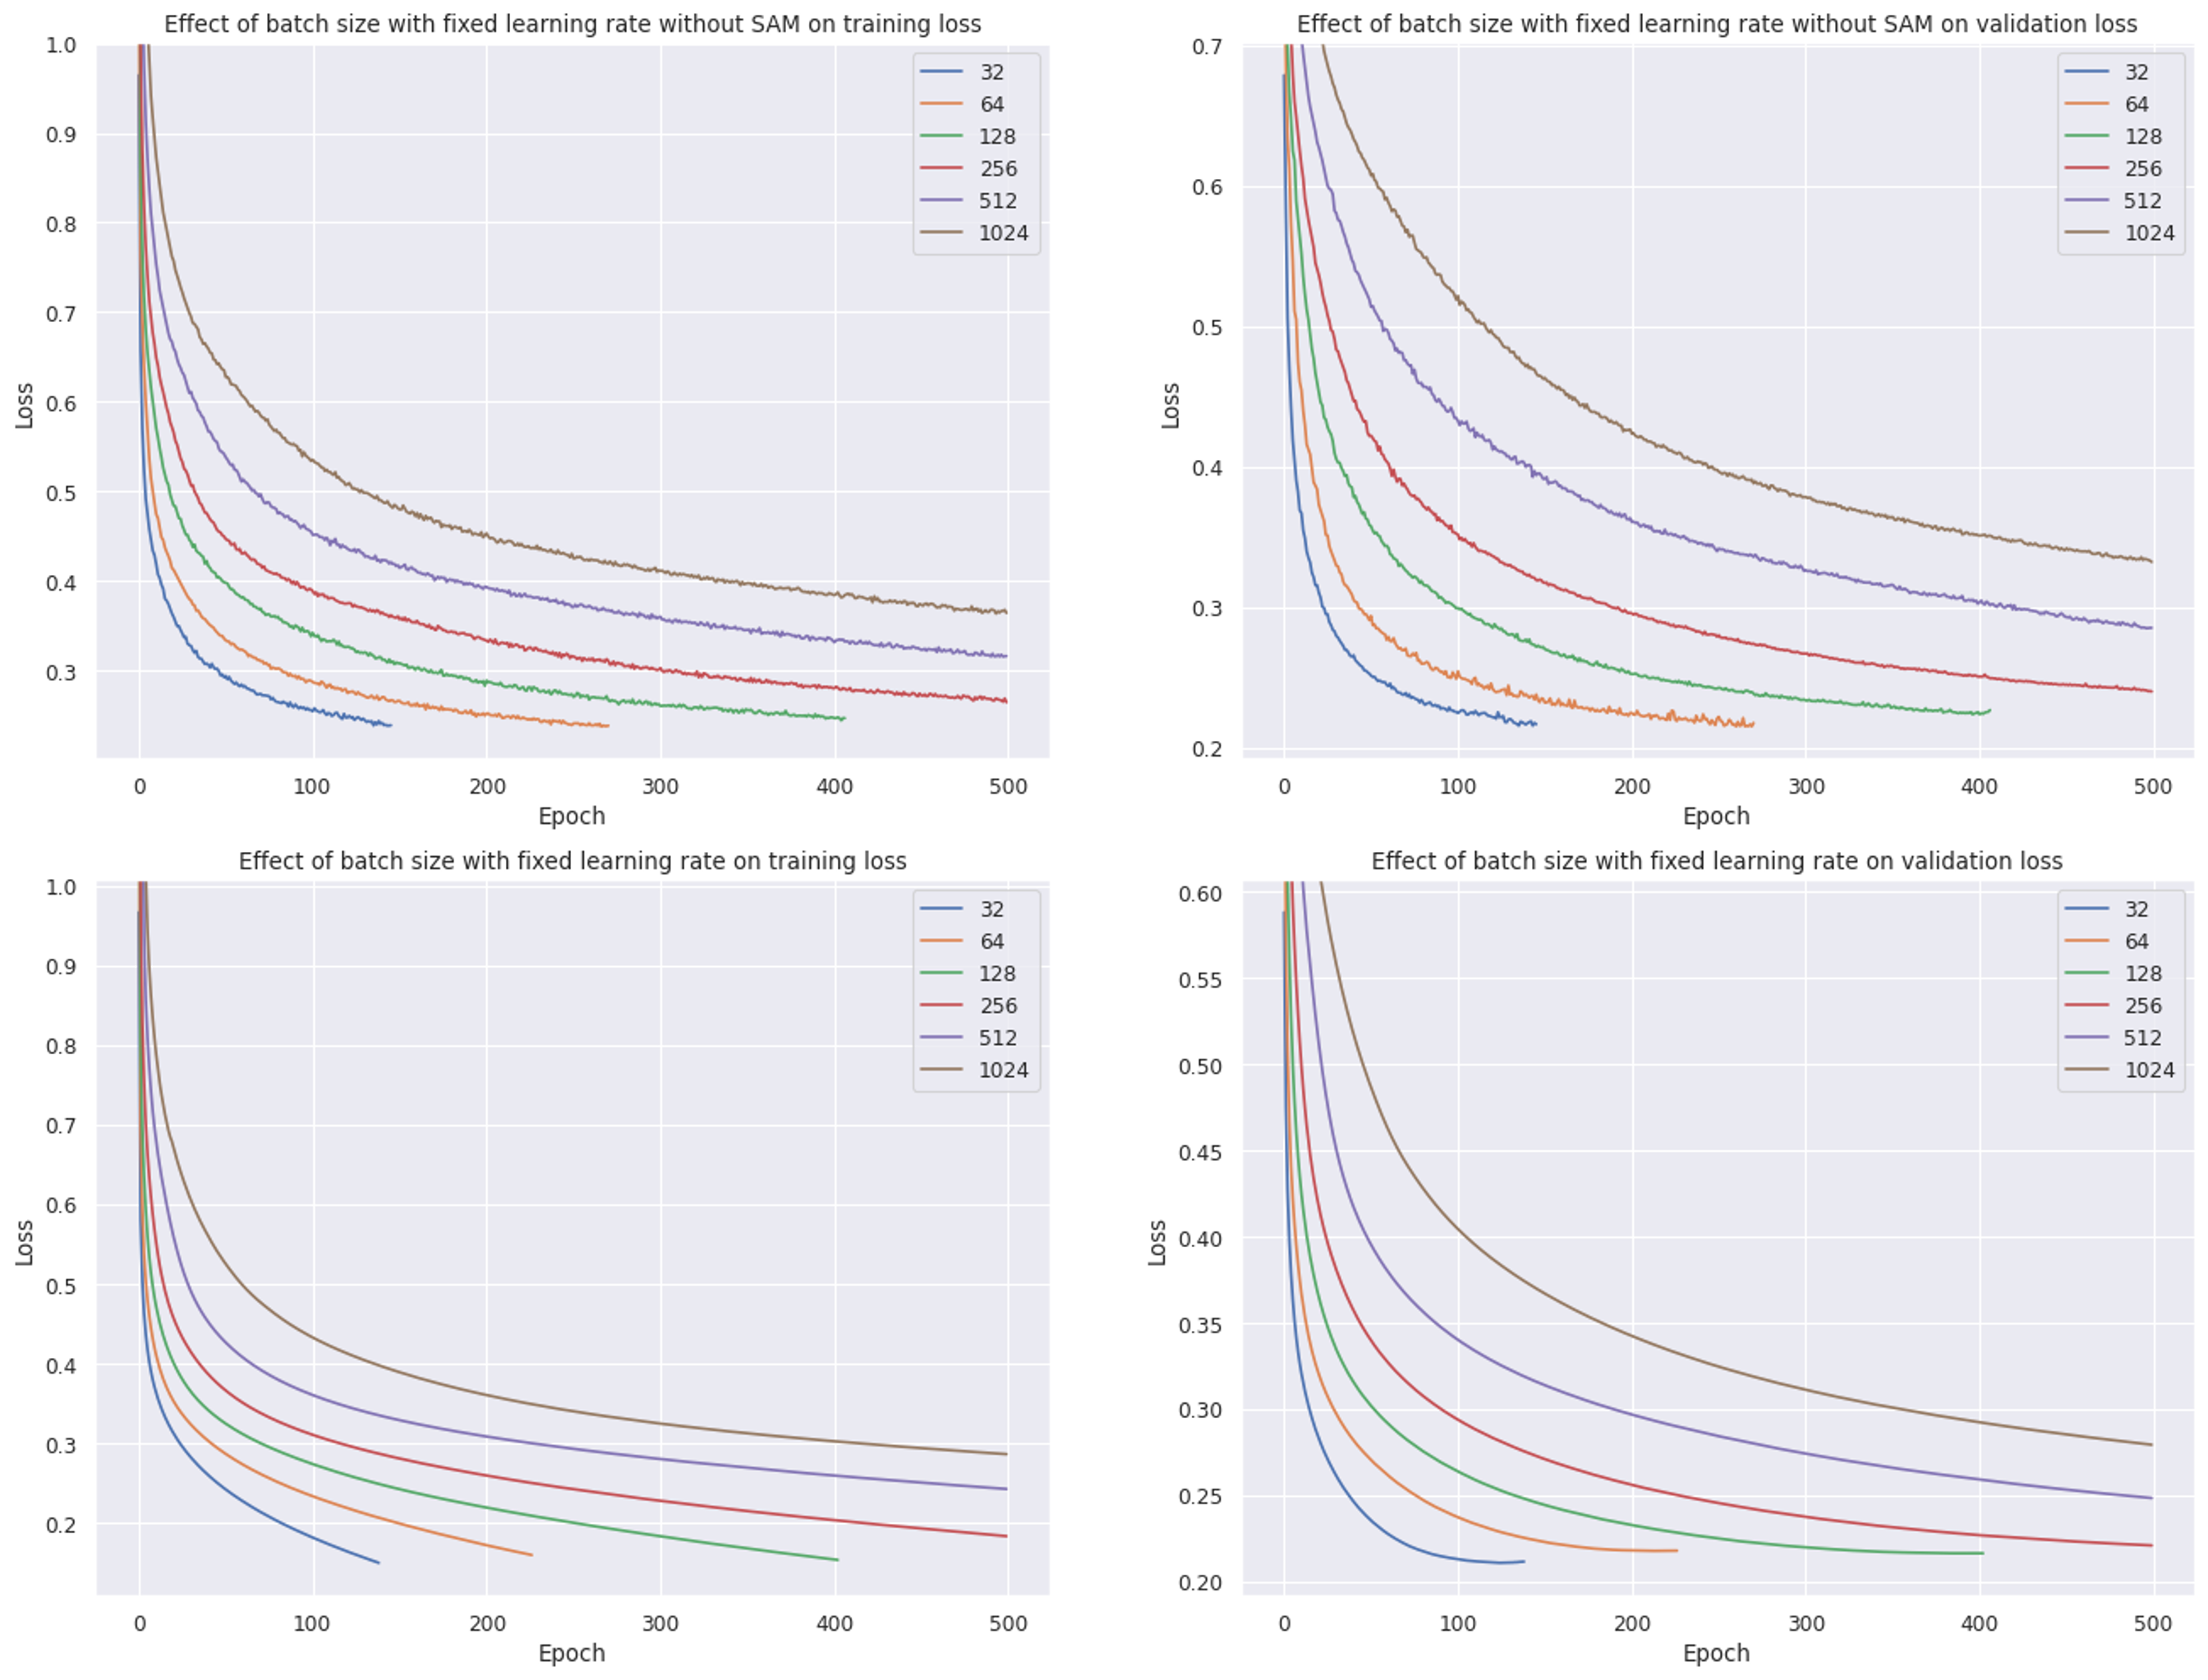
\includegraphics[width=\columnwidth]{img/figure1_val_loss_with_without_sam_sgd}
  \caption{Training and test loss for SGD with an increasing learning rate, once without (top) and once with (bottom) SAM.}
  \vspace{-3mm}
  \label{fig:val-loss-with-without}
\end{figure}
\begin{figure}[tbp]
  \centering
  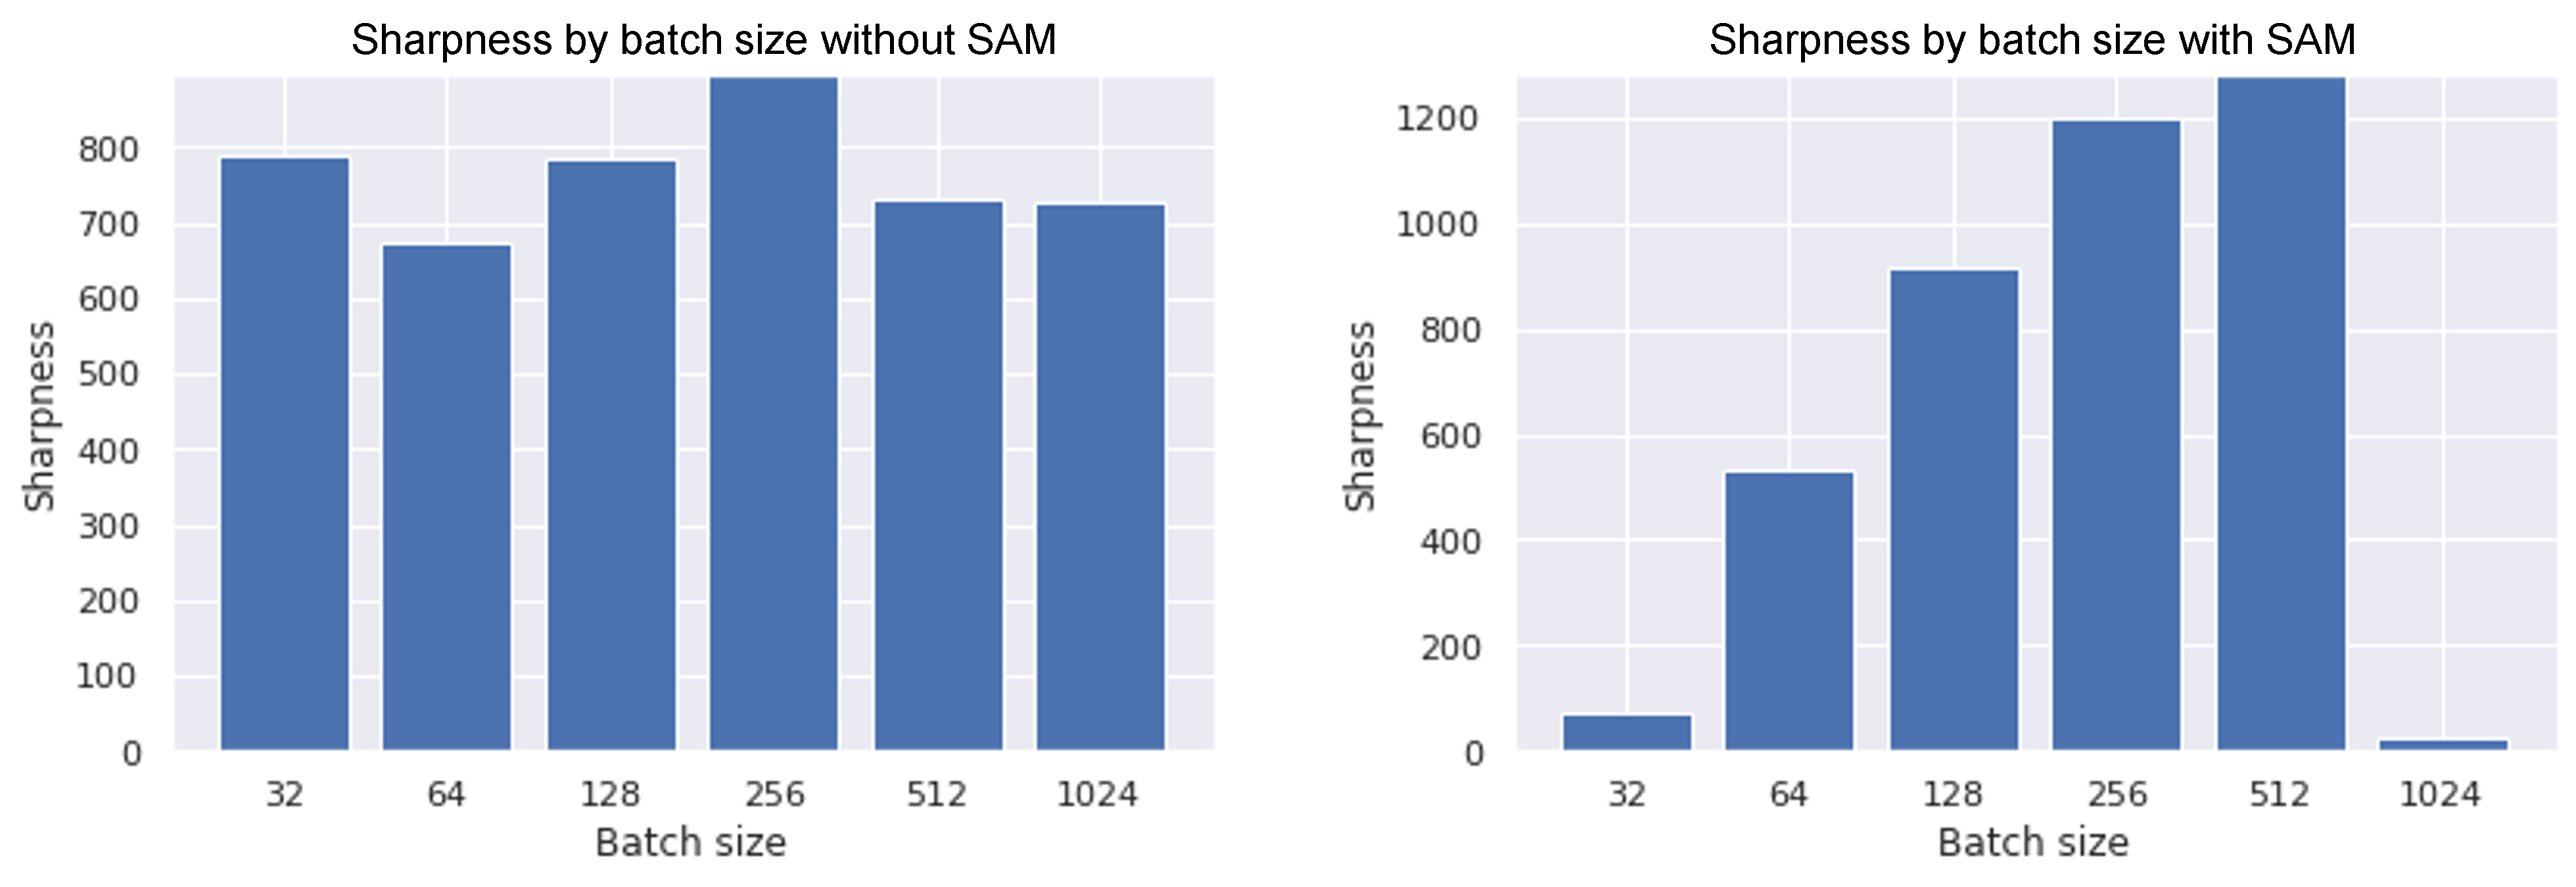
\includegraphics[width=\columnwidth]{img/figure2_sharpness_with_without_sam_sgd}
  \caption{Sharpness scores for SGD with an increasing learning rate, once without (left) and once with (right) SAM. Note the y-axis is not shared. One can see the decrease in sharpness for batch sizes 32 and 64 as well as the outlier in 1024.}
  \vspace{-3mm}
  \label{fig:sharpness-with-without}
\end{figure}
We conducted the following experiments: A simple model like described in \ref{subsec:our-observations} was trained both with a constant learning rate and with an adjusted learning rate. In both cases, we considered different batch sizes (extrema of 32 and 1024) and trained the model once with and once without SAM.

SGD-models with and increasing learning rate and SAM did in fact achieve a reduced sharpness for some batches. This reduction was strongest for batch size 32, where the sharpness was reduced by a factor of nine. For batch size 64, the sharpness was also reduced by half. However, we could no longer see any improvement for batch size 128 and the sharpness even worsened for the larger batch sizes. The largest batch size (1024) is an outlier. Here the sharpness is lowest, but the validation accuracy is also reduced (Figure \ref{fig:val-loss-with-without} and \ref{fig:sharpness-with-without}). Accordingly, this cannot generally be called a success.

\begin{figure}[tbp]
  \centering
  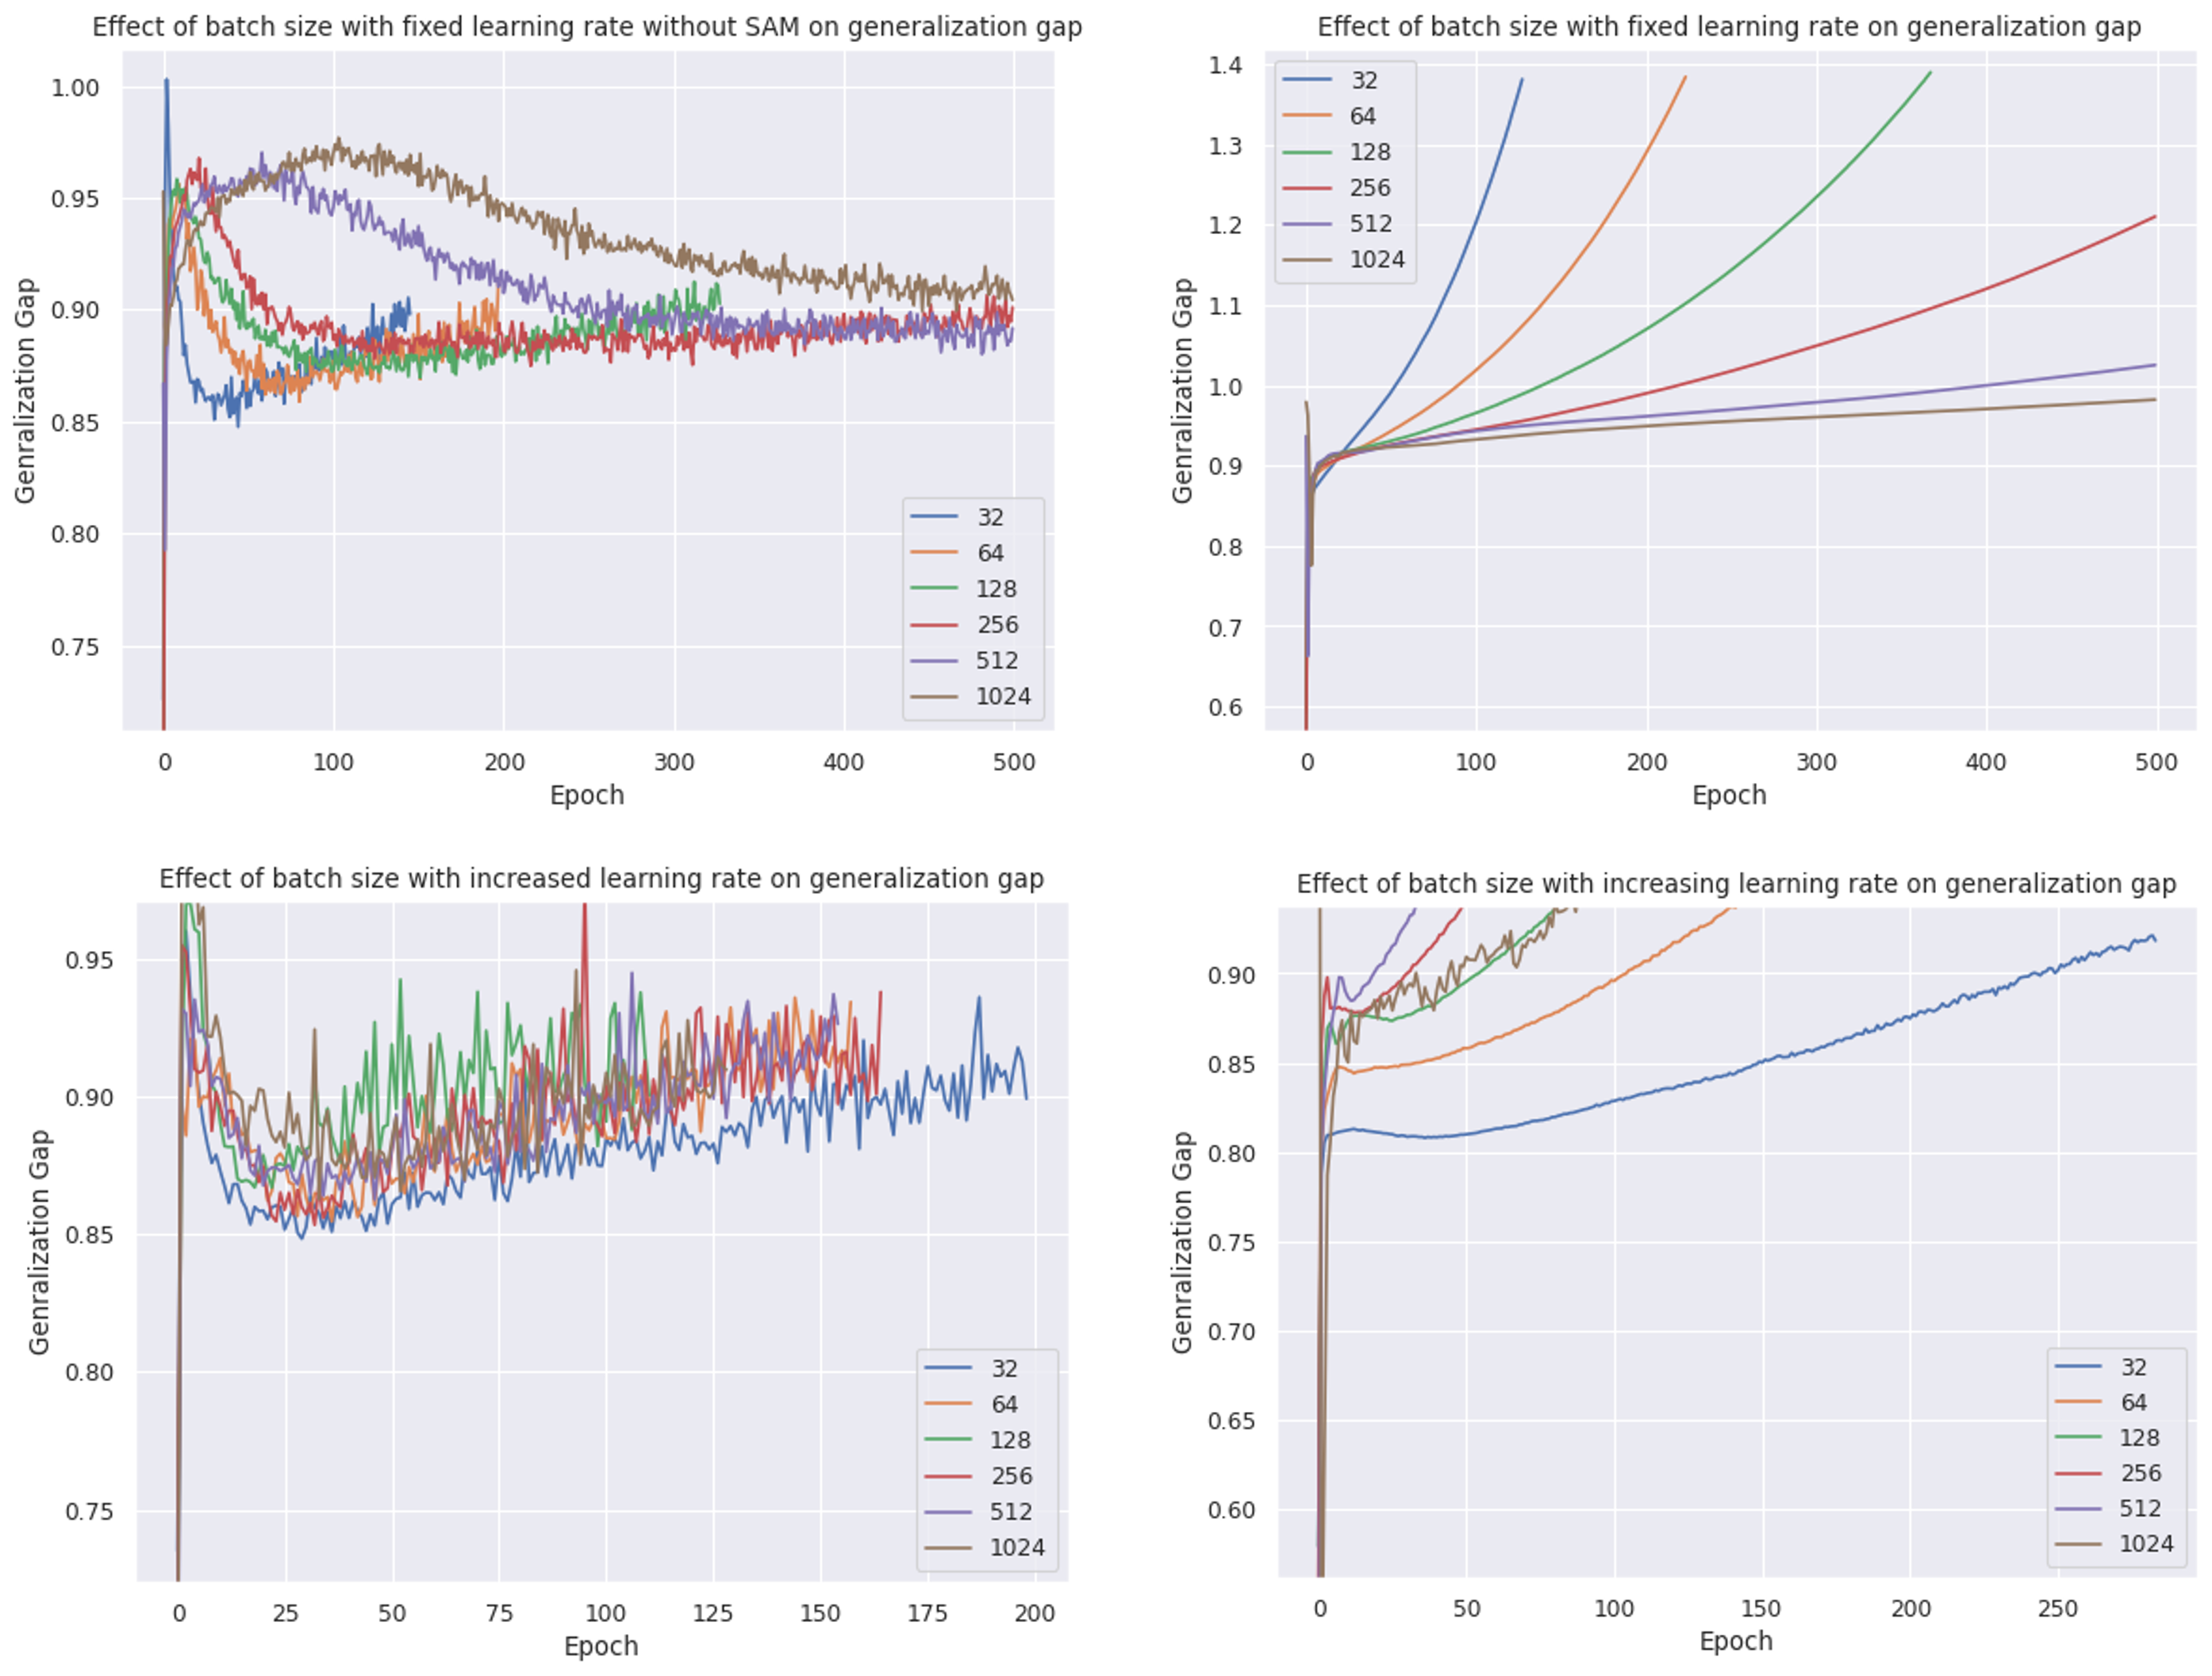
\includegraphics[width=\columnwidth]{img/figure5_gen_gap}
  \caption{Ratio of train error to test error for fixed (top) and increasing (bottom) learning rates once without (left) and once with (right) SAM.}
  \vspace{-3mm}
  \label{fig:gen-gap}
\end{figure}

Looking at the generalization gap one can see from Figure \ref{fig:gen-gap} that...

The outlier in the sharpness and the validation accuracy for batch size 1024 is interesting. We cannot provide an exact explanation for this. It is possible that the minimiser is not only in a local minimum of the function value, but also in a local minimum of the sharpness, from which it cannot break out. It would be interesting to observe in the future whether an increase in the hyperparameter rho can bring about a change here and prevent local sharpness minima. 

When using large batches, the runtime is reduced quite a bit. This is because the calculation of the gradients can be better parallelized with larger batches. This reduces the training time per epoch.

The runtime when using SAM basically doubles, regardless of the size of the batches used. This is primarily because the gradient must be calculated twice for each iteration step when using SAM.

Our tests also showed that in no scenario could an improvement be achieved by SAM when using Adam. Neither the sharpness nor the validation accuracy could be improved even when using a fixed learning rate (see Figure \ref{fig:adam-val-loss-with-without} and \ref{fig:adam-sharpness-with-without}). SAM could not provide a benefit here.

\begin{figure}[tbp]
  \centering
  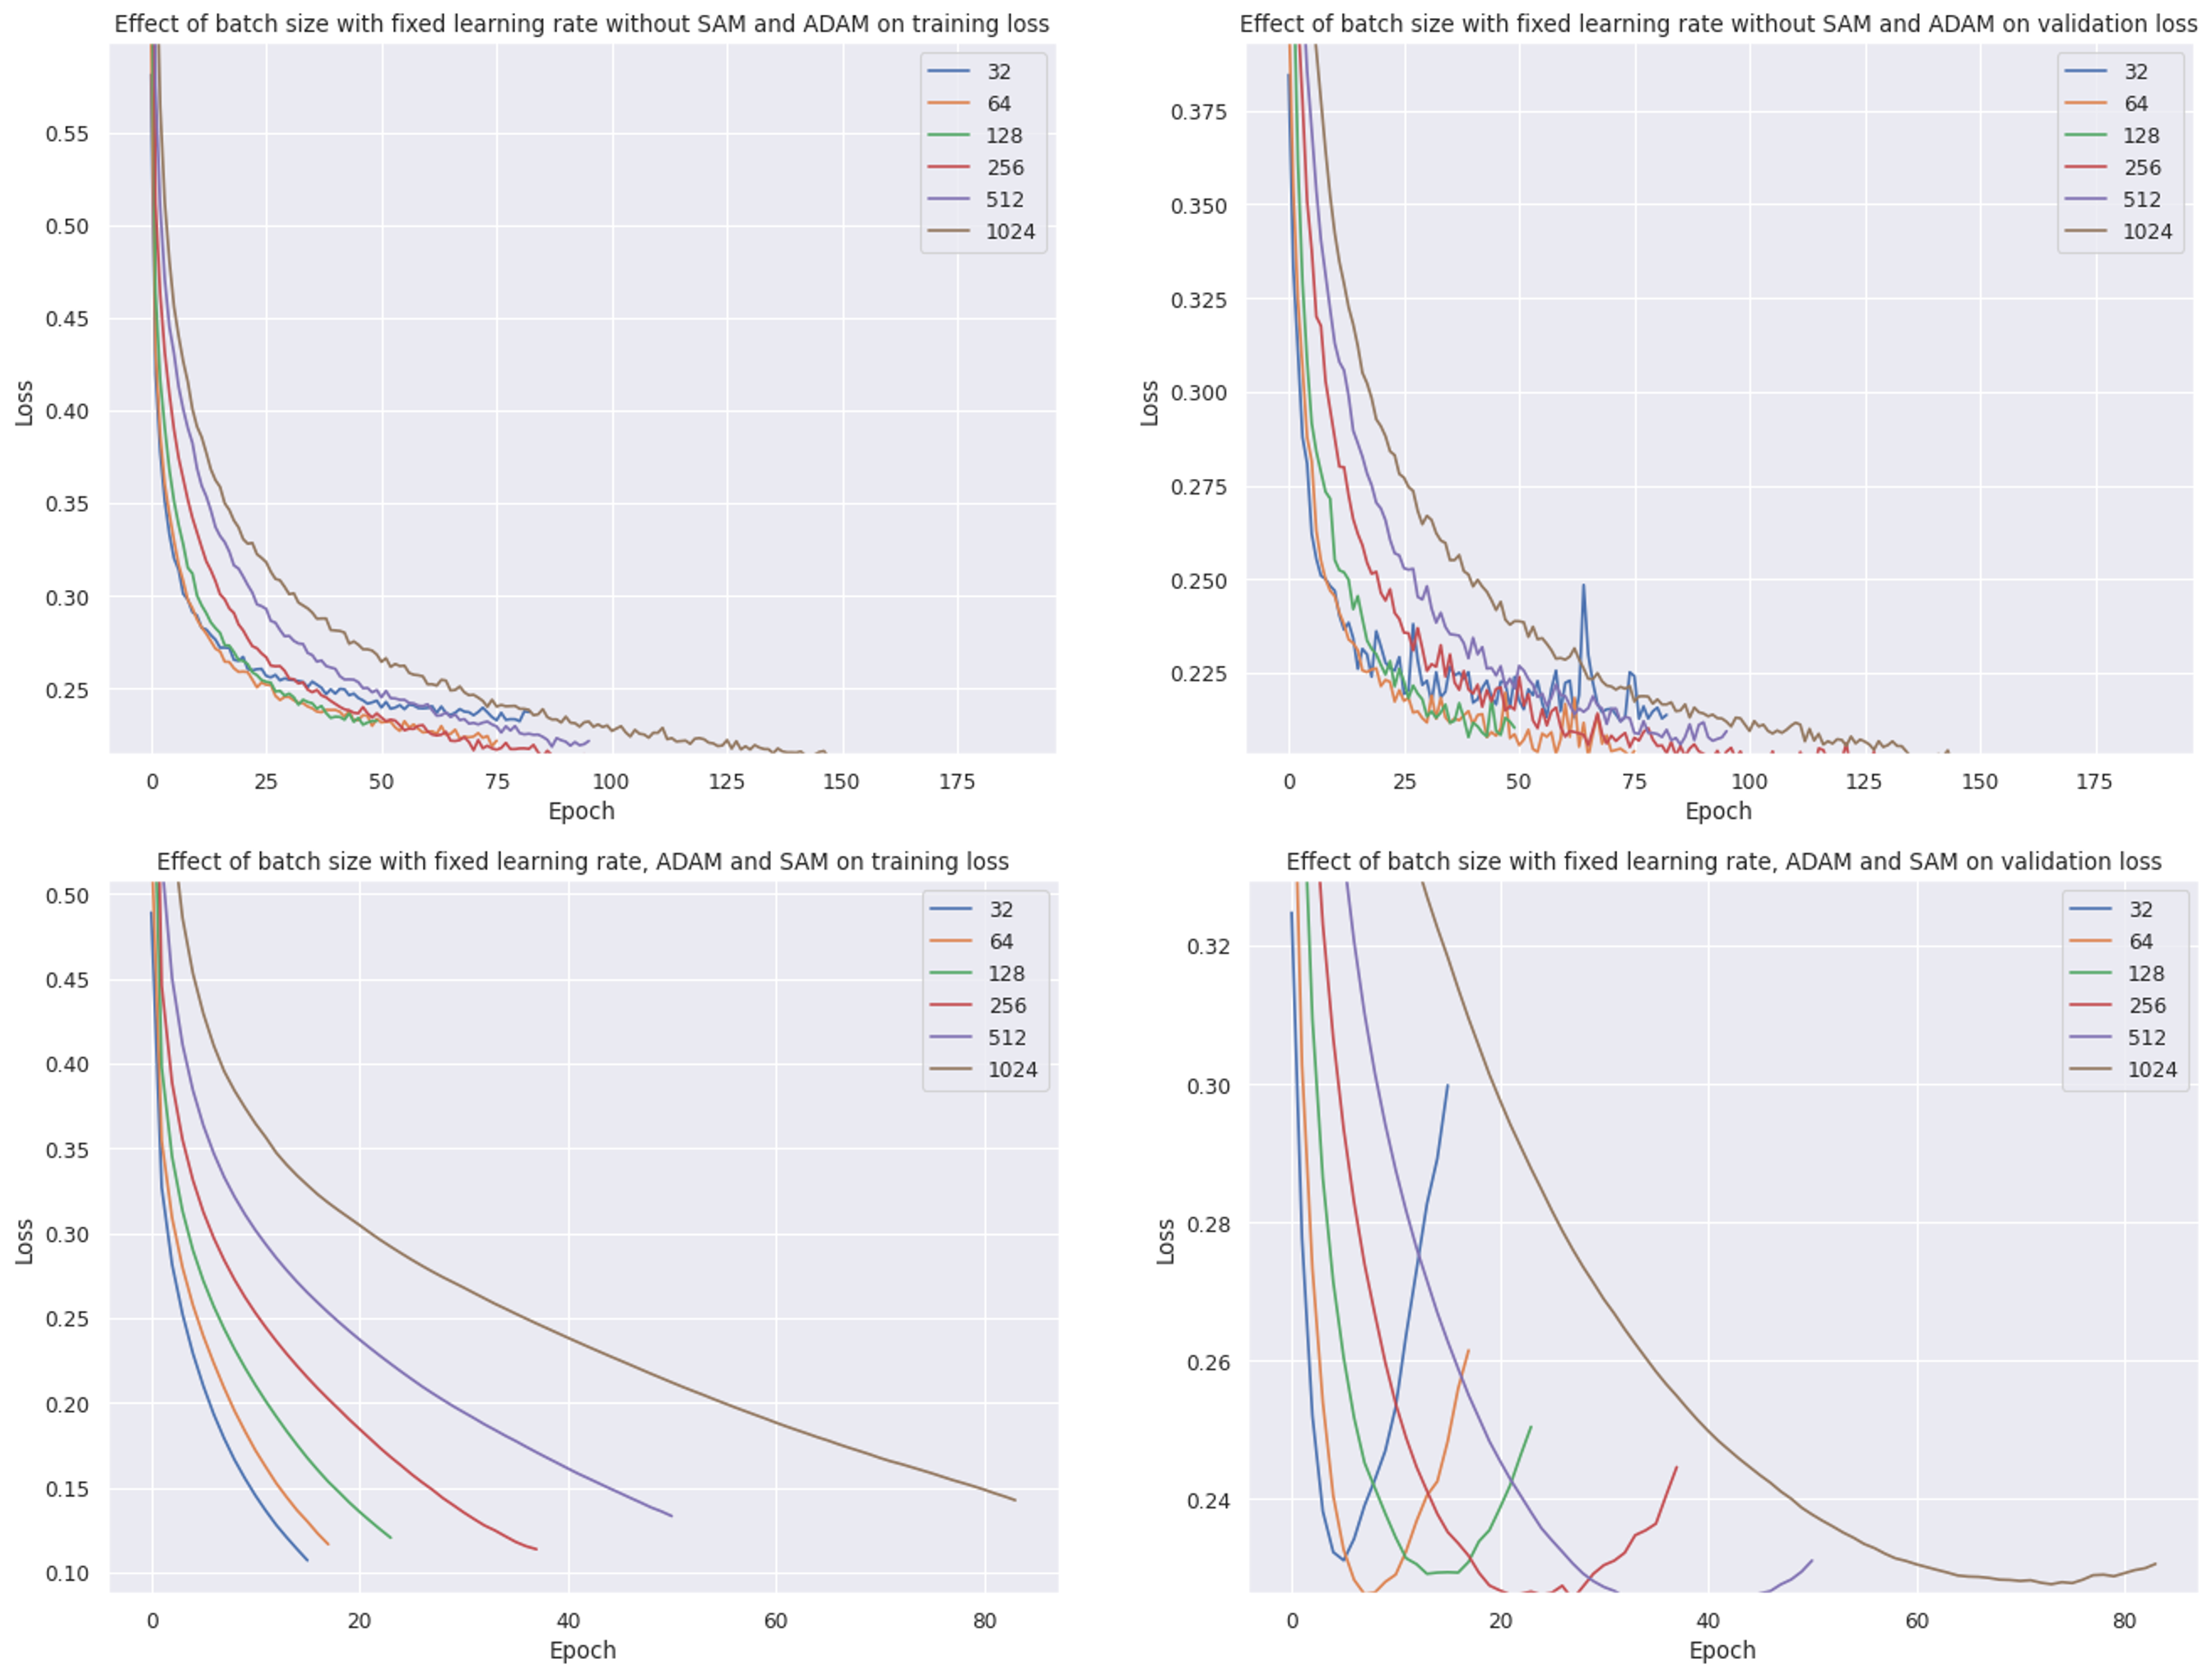
\includegraphics[width=\columnwidth]{img/figure3_val_loss_with_without_sam_adam}
  \caption{Training and test loss for Adam without (top) and with (bottom) SAM. Clearly both approaches do not yield satisfactory results.}
  \vspace{-3mm}
  \label{fig:adam-val-loss-with-without}
\end{figure}
\begin{figure}[tbp]
  \centering
  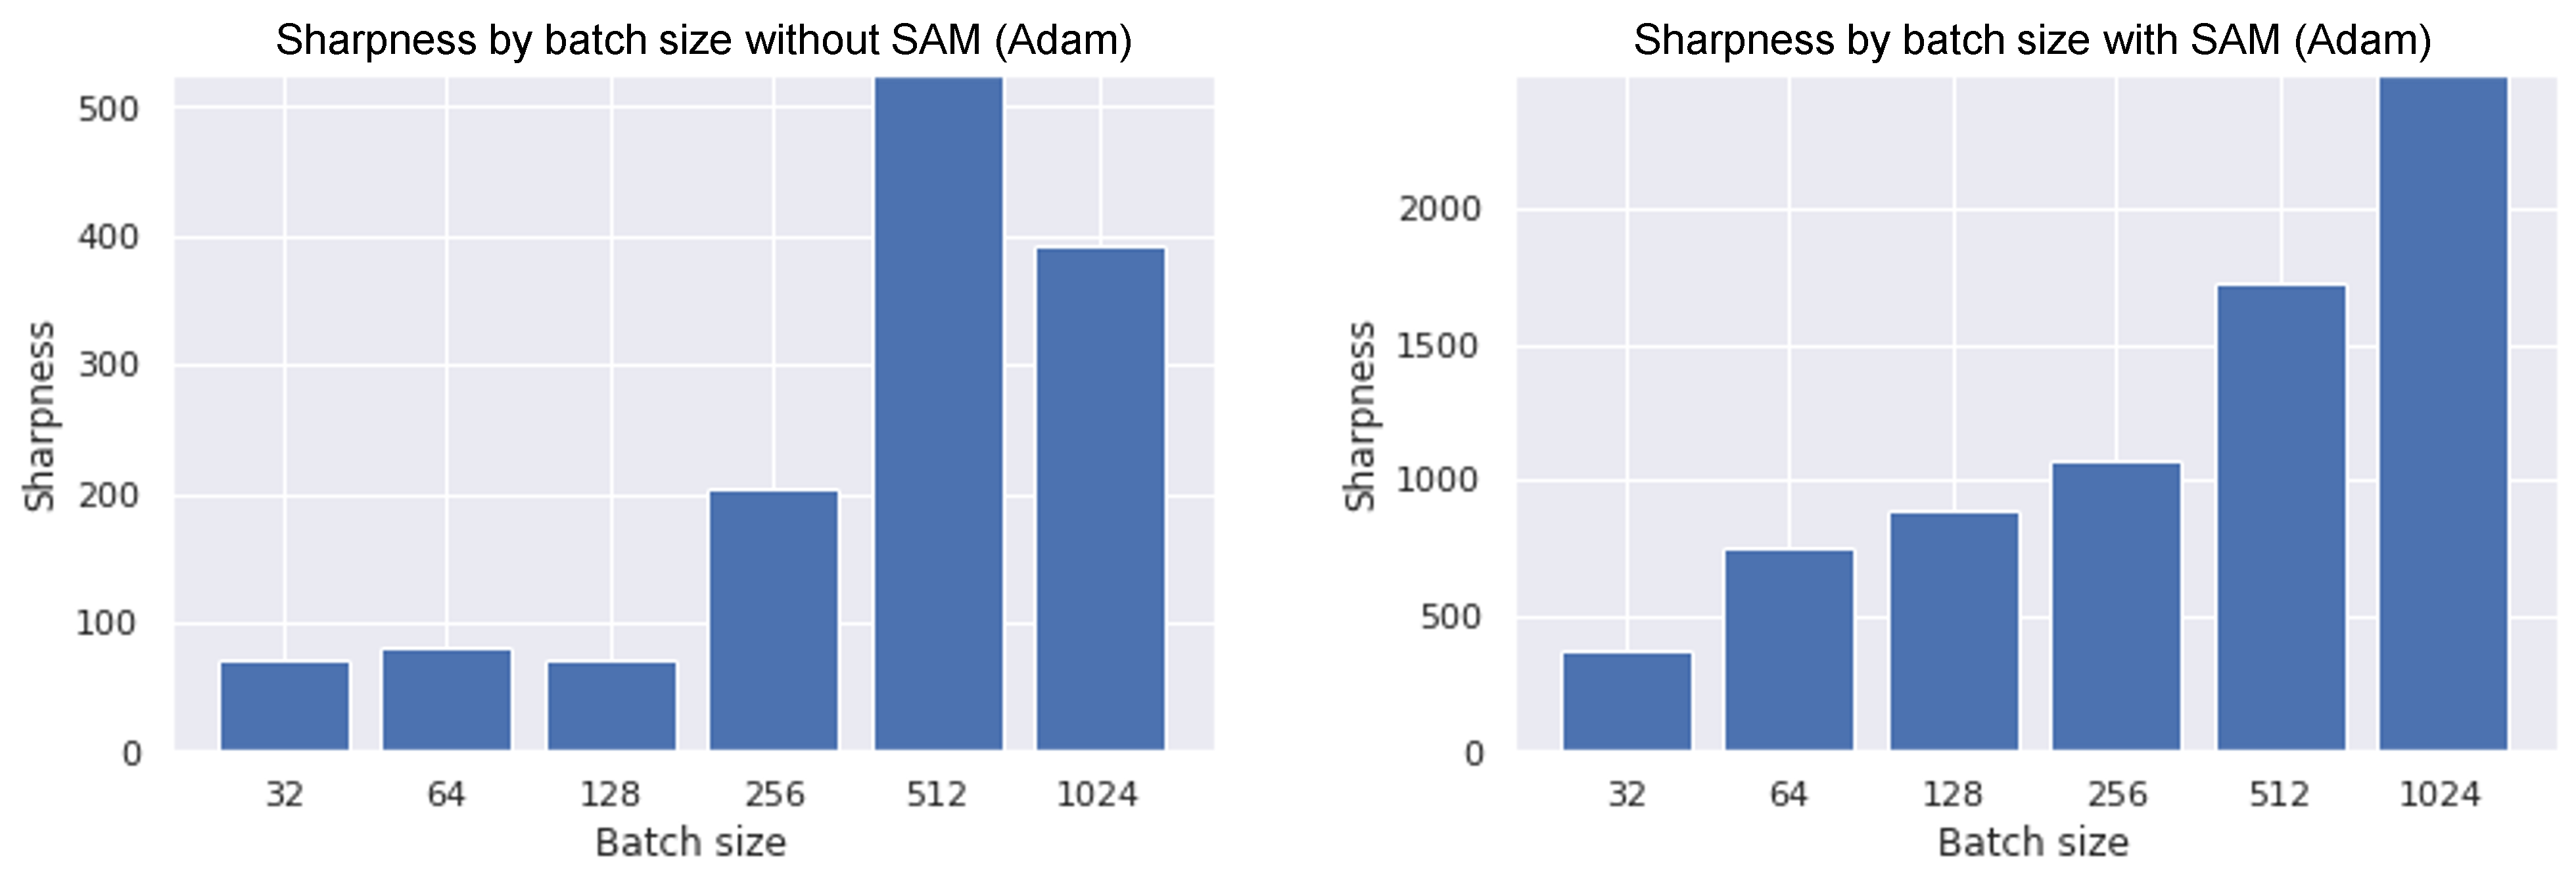
\includegraphics[width=\columnwidth]{img/figure4_sharpness_with_without_sam_adam}
  \caption{Sharpness scores for Adam without (left) and with (right) SAM. Note the y-axis is not shared.}
  \vspace{-3mm}
  \label{fig:adam-sharpness-with-without}
\end{figure}

In summary, we can say that (in our scenario) SAM, while maintaining validation accuracy, is only able to reduce sharpness at small batch sizes, i.e. {32, 64}. Therefore, it cannot be deduced from our experiments that SAM brings an advantage with large batches. On the contrary, the runtime doubles and the final validation accuracy decreases.

\section{old}
In this section we will evaluate our results. Note that for all the results in this section we use an increasing learning rate for the respective optimizer. At first we will look at the validation loss of SGD with and without SAM. Surprisingly enough the model with SAM seems to perform worse on the test set than without (see figure \ref{fig:val-loss-with-without}). This is not surprising considering the fact that the minima are even sharper when using SAM for large batch sizes (see figure \ref{fig:sharpness-with-without}). Why we don't observe flatter minima is up for further investigation as we are using the almost unchanged (except the base model) implementation of \cite{paulSharpnessAwareMinimizationTensorFlow2022}.


Using different variants of SGD worsened the results even more as can be seen in Figure \ref{fig:adam-val-loss-with-without} and Figure \ref{fig:adam-sharpness-with-without} for Adam.



\section{Summary}

Since large batch sizes often suffer from a larger generalization gap we tried to investigate the causes of this phenomena. As a result we focussed on achieving flatter minima as this seems to be a deviance between small and large batch sizes. We apply a solution in form of Sharpness-Aware-Minimization (SAM) to evaluate if SAM can be used to circumvent this issue. We found that although there are some cases where the sharpness is reduced, we could not achieve flatter minima in large batch training. The sharpness score rather increased than decreased. This result suggests that at least for our architecture and setting SAM does not provide an advantage since its runtime is roughly twice as large as without SAM.




\newpage
\bibliographystyle{IEEEtran}
\bibliography{literature}

\newpage
\section*{Appendix}
\label{sec:appendix}
Additional plots for the conducted experiments:
\begin{figure}[H]
  \centering
  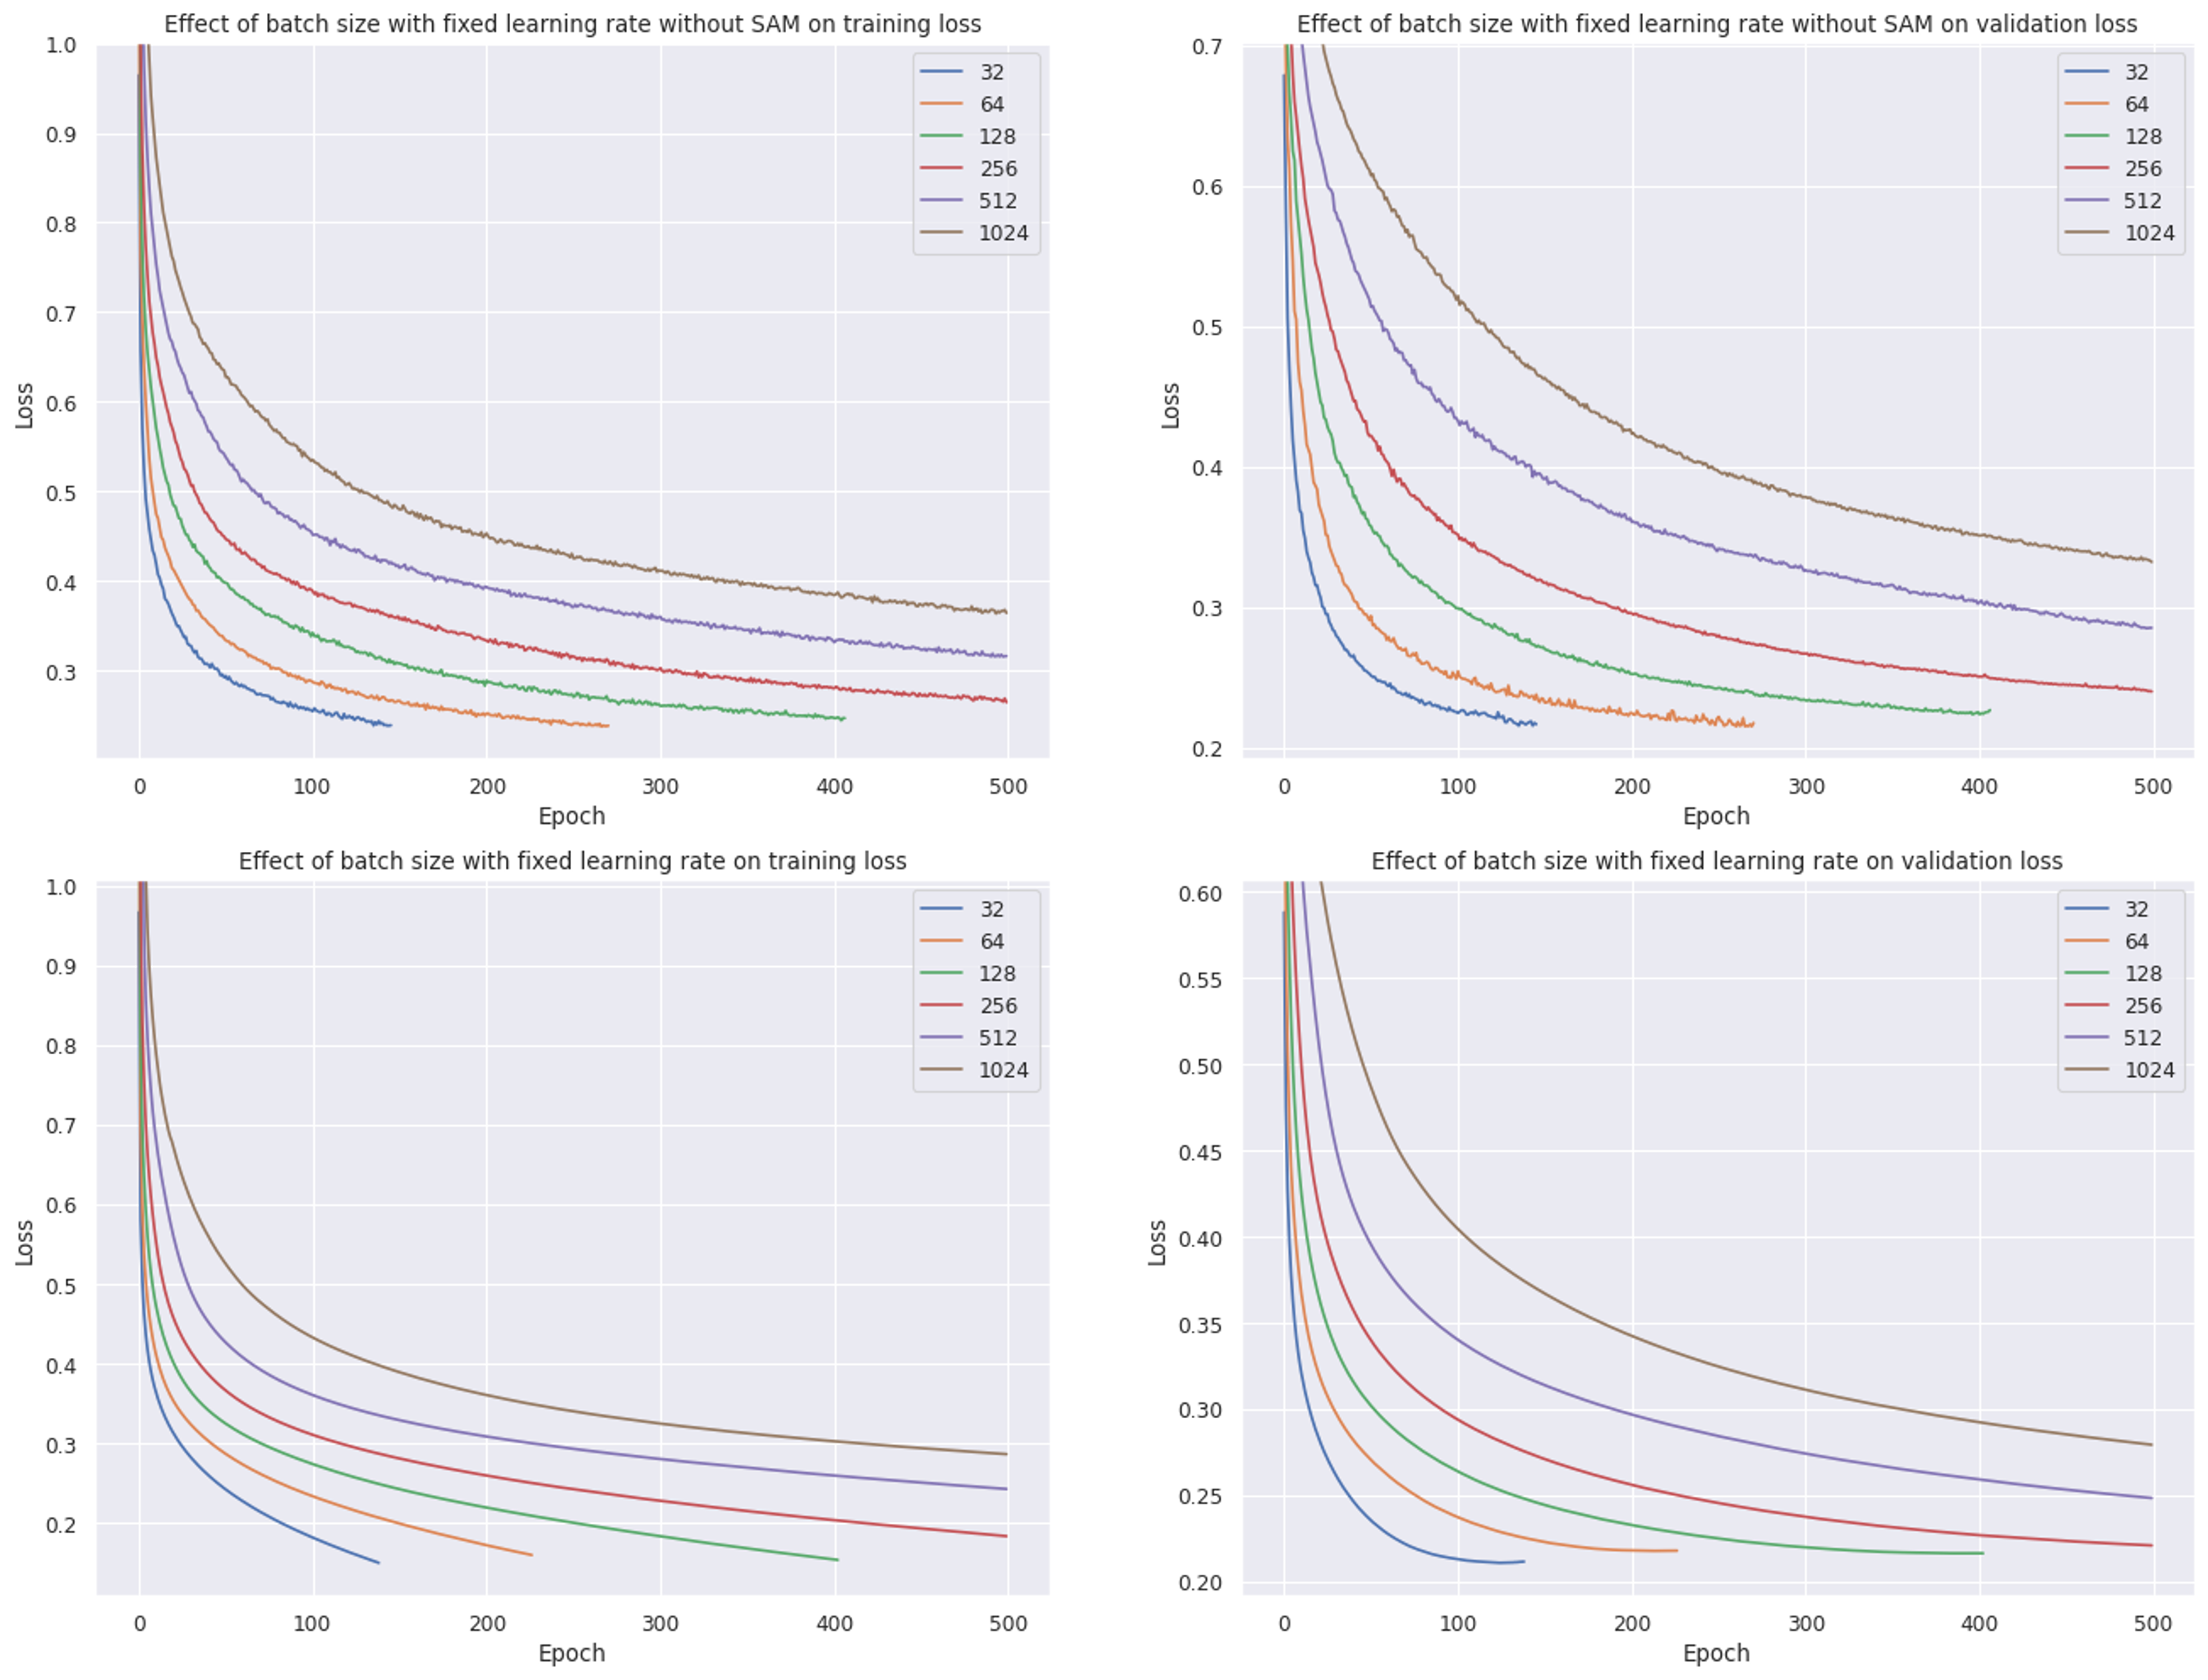
\includegraphics[width=\columnwidth]{img/figure6_val_loss_with_without_sam_sgd_FIXED_LR}
  \caption{Training and test loss for SGD without (top) and with (bottom) SAM with a fixed learning rate}
  \vspace{-3mm}
  \label{fig:adam-val-loss-with-without-fixed}
\end{figure}
\begin{figure}[H]
  \centering
  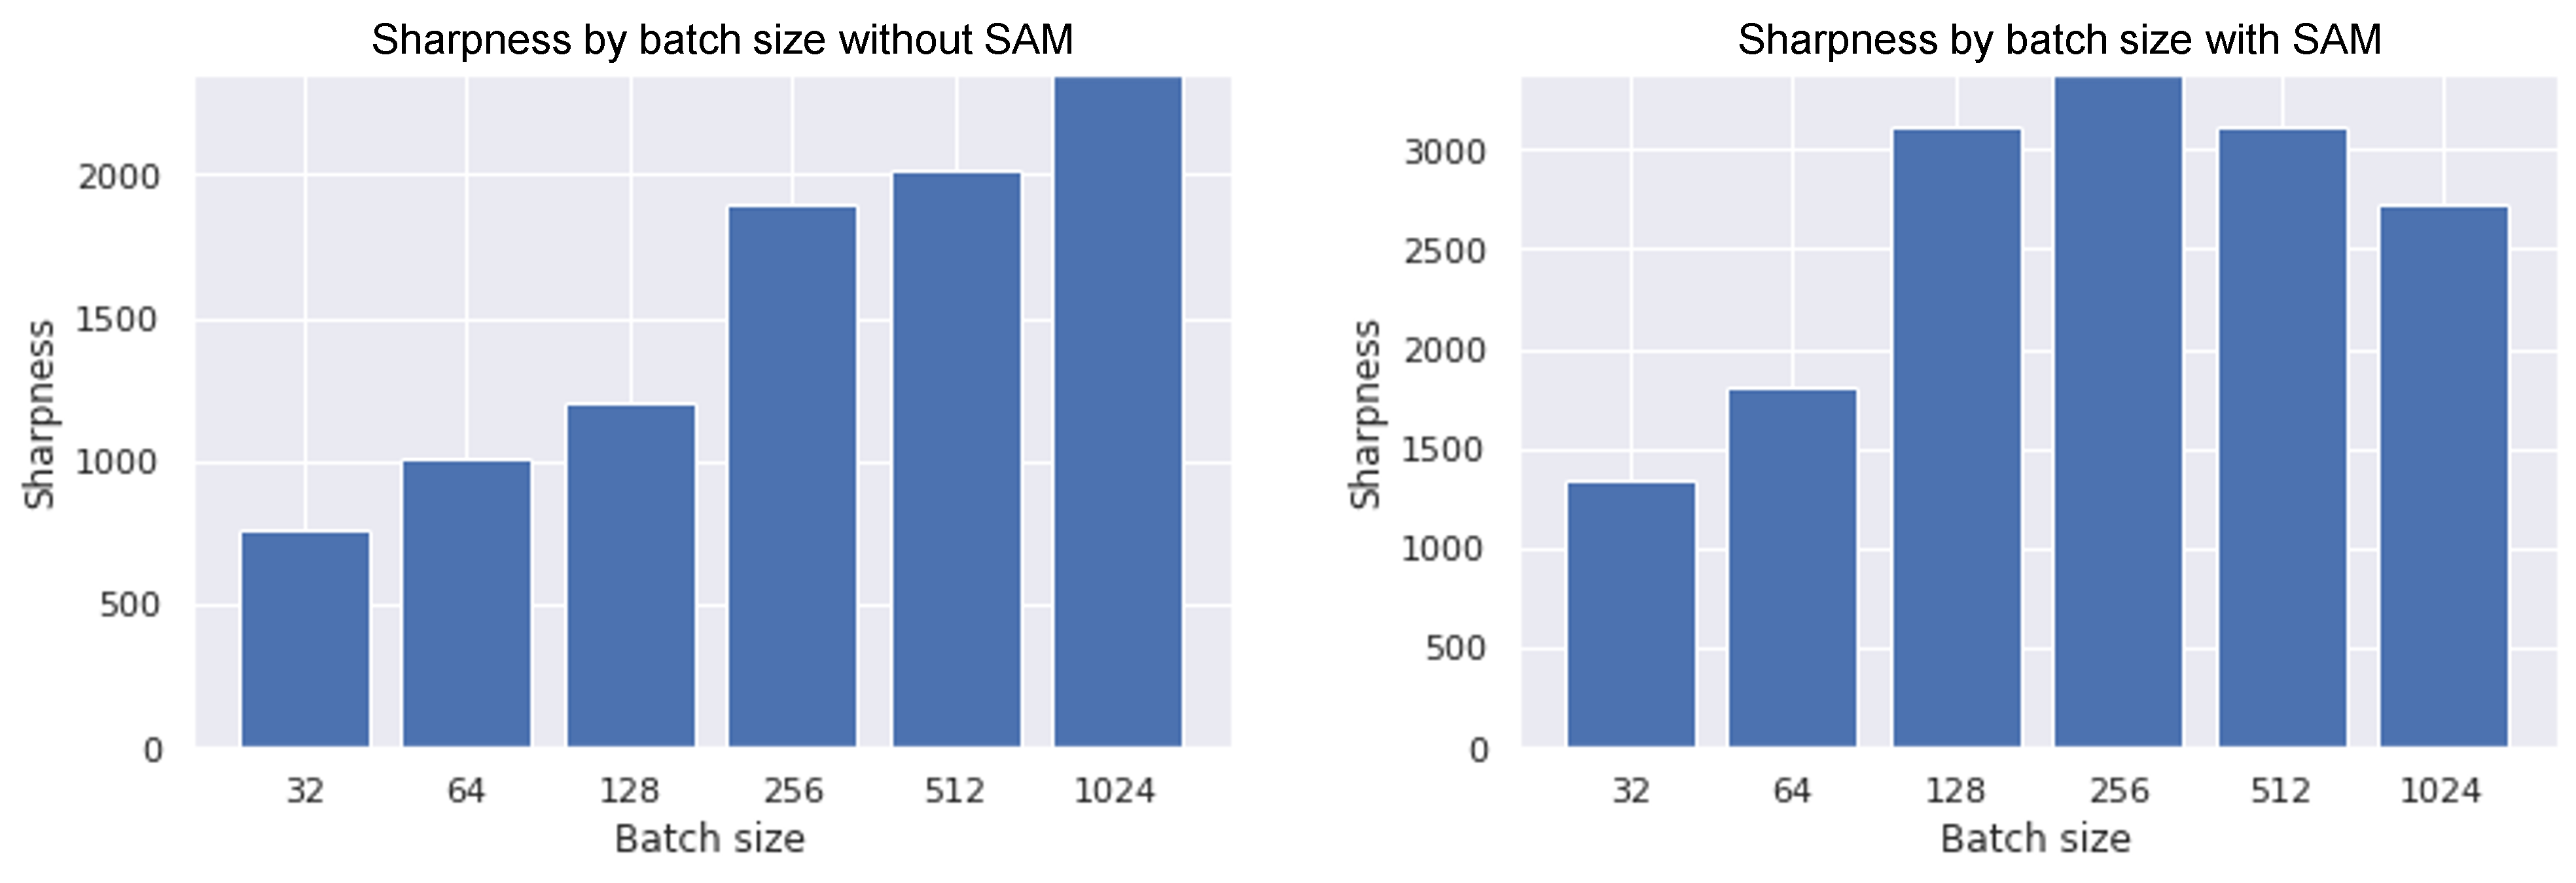
\includegraphics[width=\columnwidth]{img/figure7_sharpness_with_without_sam_sgd_FIXED_LR}
  \caption{Sharpness scores for SGD without (left) and with (right) SAM for a fixed learning rate. Note the y-axis is not shared.}
  \vspace{-3mm}
  \label{fig:adam-sharpness-with-without-fixed}
\end{figure}
\end{document}
